\chapter{Результати адаптивних алгоритмів}

\section{Проста тестова задача}

\begin{figure}[H]
    \centering
    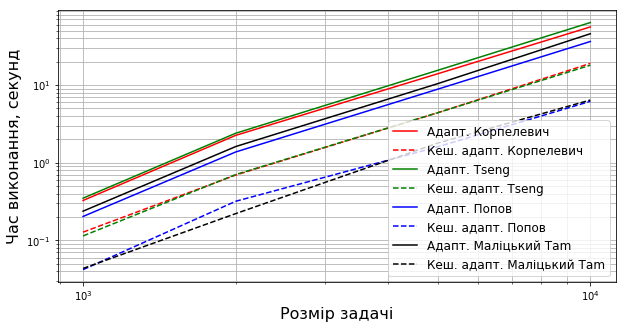
\includegraphics[width=.75\textwidth]{img/1/adapt/time.png}
\end{figure}

Та сама інформація у табличці, для зручності:

\begin{table}[H]
	\centering
	\begin{tabular}{|c||c|c|c|c|}\hline
		Розмір задачі & 1000 & 2000 & 5000 & 10000 \\ \hline \hline
		Корпелевич & 0.11 & 0.65 & 4.95 & 19.31 \\ \hline
		Tseng & 0.10 & 0.98 & 7.13 & 26.82 \\ \hline
		Кеш. Tseng & 0.07 & 0.71 & 4.49 & 17.98 \\ \hline
		Попов & 0.08 & 0.50 & 2.98 & 12.18 \\ \hline
		Кеш. Попов & 0.03 & 0.26 & 1.52 & 6.16 \\ \hline \hline
		Адапт. Корпелевич & 0.21 & 1.71 & 12.70 & 50.57 \\ \hline
		Кеш. адапт. Корпелевич & 0.11 & 0.56 & 4.15 & 16.89 \\ \hline
		Адапт. Tseng & 0.27 & 1.91 & 14.58 & 58.36 \\ \hline
		Кеш. адапт. Tseng & 0.07 & 0.57 & 4.16 & 16.69 \\ \hline
		Адапт. Попов & 0.31 & 2.45 & 17.84 & 73.44 \\ \hline
		Кеш. адапт. Попов & 0.07 & 0.54 & 3.03 & 12.29 \\ \hline
	\end{tabular}
	\caption{Час виконання, секунд}
\end{table}


Алгоритма Попова програє своїй неадаптивній версії. Окрім цього, некешовані версії адаптивних алгоритмів явно програють кешованим. Кешовані версії адаптивних алгоритмів Корпелевич і Tseng'a не поступаються кешованим неадаптивним версіям. \medskip

Щодо кількості ітерацій ситуація схожа:

\begin{table}[H]
	\centering
	\begin{tabular}{|c||c|c|c|c|}\hline
		Розмір задачі & 1000 & 2000 & 5000 & 10000 \\ \hline \hline
		Адапт. Корпелевич & 125 & 129 & 135 & 139 \\ \hline
		Кеш. адапт. Корпелевич & 125 & 129 & 135 & 139 \\ \hline
		Адапт. Tseng & 125 & 129 & 135 & 139 \\ \hline
		Кеш. адапт. Tseng & 125 & 129 & 135 & 139 \\ \hline
		Адапт. Попов & 179 & 185 & 194 & 201 \\ \hline
		Кеш. адапт. Попов & 179 & 185 & 194 & 201 \\ \hline
	\end{tabular}
	\caption{Число ітерацій}
\end{table}


\section{Проста тестова задача із розрідженими матрицями}

\begin{figure}[H]
    \centering
    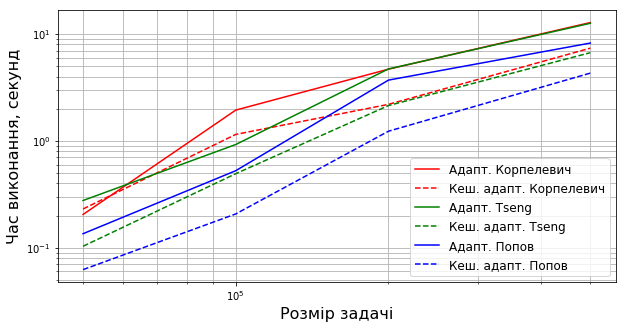
\includegraphics[width=.75\textwidth]{img/1/sparse/adapt/time.png}
\end{figure}

Та сама інформація у табличці:

\begin{table}[H]
	\centering
	\begin{tabular}{|c||c|c|c|c|}\hline
		Розмір задачі & 50000 & 100000 & 200000 & 500000 \\ \hline \hline
		Корпелевич & 0.07 & 0.23 & 2.23 & 5.28 \\ \hline
		Tseng & 0.13 & 0.53 & 1.96 & 6.97 \\ \hline
		Кеш. Tseng & 0.09 & 0.24 & 1.75 & 5.69 \\ \hline
		Попов & 0.06 & 0.12 & 1.58 & 3.91 \\ \hline
		Кеш. Попов & 0.04 & 0.25 & 0.86 & 2.09 \\ \hline
		Маліцький Tam & 0.07 & 0.26 & 1.33 & 5.09 \\ \hline
		Кеш. Маліцький Tam & 0.04 & 0.10 & 0.91 & 3.76 \\ \hline \hline
		Адапт. Корпелевич & 0.27 & 0.95 & 4.85 & 13.73 \\ \hline
		Кеш. адапт. Корпелевич & 0.11 & 1.07 & 2.41 & 7.64 \\ \hline
		Адапт. Tseng & 0.20 & 1.20 & 4.65 & 14.15 \\ \hline
		Кеш. адапт. Tseng & 0.11 & 0.62 & 3.19 & 7.31 \\ \hline
		Адапт. Попов & 0.24 & 0.68 & 3.54 & 9.67 \\ \hline
		Кеш. адапт. Попов & 0.07 & 0.17 & 2.14 & 4.35 \\ \hline
		Адапт. Маліцький Tam & 0.14 & 0.37 & 3.14 & 9.35 \\ \hline
		Кеш. адапт. Маліцький Tam & 0.09 & 0.13 & 1.81 & 4.73 \\ \hline
	\end{tabular}
	\caption{Час виконання, секунд}
\end{table}


\begin{table}[H]
	\centering
	\begin{tabular}{|c||c|c|c|c|}\hline
		Розмір задачі & 50000 & 100000 & 200000 & 500000 \\ \hline \hline
		Адапт. Корпелевич & 256 & 261 & 266 & 272 \\ \hline
		Кеш. адапт. Корпелевич & 256 & 261 & 266 & 272 \\ \hline
		Адапт. Tseng & 256 & 261 & 266 & 272 \\ \hline
		Кеш. адапт. Tseng & 224 & 229 & 234 & 240 \\ \hline
		Адапт. Попов & 149 & 152 & 155 & 159 \\ \hline
		Кеш. адапт. Попов & 149 & 152 & 155 & 159 \\ \hline
		Адапт. Маліцький Tam & 171 & 175 & 178 & 182 \\ \hline
		Кеш. адапт. Маліцький Tam & 171 & 175 & 178 & 182 \\ \hline
	\end{tabular}
	\caption{Число ітерацій}
\end{table}


Ситуація доволі схожа на попередню, за виключення того що алгоритм Попва тепер не так суттєво програє неадаптивній версії.

\section{Середня тестова задача}

\begin{figure}[H]
    \centering
    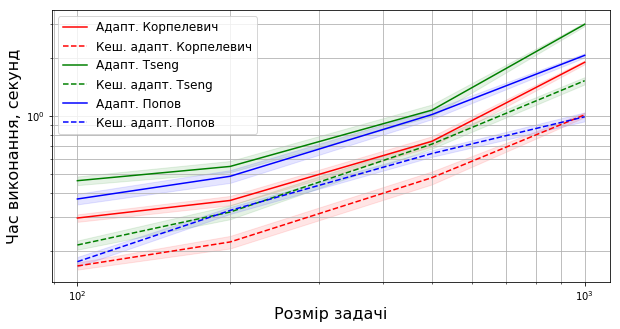
\includegraphics[width=.75\textwidth]{img/2/adapt/time.png}
\end{figure}

Та сама інформація у табличці:

\begin{table}[H]
	\centering
	\begin{tabular}{|c||c|c|c|c|}\hline
		Розмір задачі & 100 & 200 & 500 & 1000 \\ \hline \hline
		Адапт. Корпелевич & 0.69 $\pm$ 0.12 & 0.99 $\pm$ 0.13 & 1.70 $\pm$ 0.10 & 3.79 $\pm$ 0.15 \\ \hline
		Кеш. адапт. Корпелевич & 0.42 $\pm$ 0.08 & 0.68 $\pm$ 0.10 & 1.39 $\pm$ 0.07 & 2.56 $\pm$ 0.07 \\ \hline
		Адапт. Tseng & 0.86 $\pm$ 0.02 & 0.98 $\pm$ 0.01 & 1.42 $\pm$ 0.02 & 3.08 $\pm$ 0.11 \\ \hline
		Кеш. адапт. Tseng & 0.49 $\pm$ 0.09 & 0.80 $\pm$ 0.07 & 1.72 $\pm$ 0.19 & 3.49 $\pm$ 0.29 \\ \hline
		Адапт. Попов & 0.82 $\pm$ 0.19 & 1.19 $\pm$ 0.18 & 2.12 $\pm$ 0.33 & 4.78 $\pm$ 0.51 \\ \hline
		Кеш. адапт. Попов & 0.45 $\pm$ 0.09 & 0.76 $\pm$ 0.11 & 1.46 $\pm$ 0.19 & 2.65 $\pm$ 0.28 \\ \hline
		Адапт. Маліцький Tam & 0.87 $\pm$ 0.02 & 0.99 $\pm$ 0.03 & 1.39 $\pm$ 0.03 & 3.02 $\pm$ 0.02 \\ \hline
		Кеш. адапт. Маліцький Tam & 0.33 $\pm$ 0.02 & 0.45 $\pm$ 0.01 & 0.79 $\pm$ 0.01 & 1.35 $\pm$ 0.00 \\ \hline
	\end{tabular}
	\caption{Час виконання, секунд}
\end{table}


Адаптивні версії суттєво випереджають неадаптивні, причому за числом ітерацій також:

\begin{table}[H]
	\centering
	\begin{tabular}{|c||c|c|c|c|}\hline
		Розмір задачі & 100 & 200 & 500 & 1000 \\ \hline \hline
		Адапт. Корпелевич & 317 $\pm$ 66 & 359 $\pm$ 42 & 410 $\pm$ 34 & 451 $\pm$ 46 \\ \hline
		Адапт. Tseng & 504 $\pm$ 50 & 684 $\pm$ 38 & 872 $\pm$ 73 & 994 $\pm$ 68 \\ \hline
		Адапт. Попов & 430 $\pm$ 93 & 507 $\pm$ 64 & 551 $\pm$ 48 & 606 $\pm$ 57 \\ \hline
		Адапт. Маліцький Tam & 540 $\pm$ 93 & 599 $\pm$ 70 & 633 $\pm$ 52 & 647 $\pm$ 42 \\ \hline
	\end{tabular}
	\caption{Число ітерацій}
\end{table}

